\chapter{Elektronika a~tištěné spoje}
Všechny prototypy základních desekPROTOPlantu byly založeny na univerzálních tištěných spojích. Vzhledem k~tomu, že jsem po stránce vzhledu i funkčnosti nebyl s~takovýmto provedením spokojen, rozhodl jsem se nechat vyrobit vlastní tištěné spoje pro základní desku i senzorové moduly.
Díky tomuto jsem se naučil návrhu tištěných spojů a~tvorbě výrobních podkladů v~programu Autodesk EAGLE.

\section{PPMB32 -- Základní deska}
\label{subsec:motherBoard}
Základní deska je rozdělena do několika částí. 
Vzhledem k~tomu, že umím pájet velmi dobře, rozhodl jsem se pro ruční osazení všech součástek, které byly doposud osazeny pouze na různých modulech připojených k~základní desce, včetně procesoru ESP32-WROOM32D.
Z~důvodu přehlednosti jsem desku rozdělil do několika částí:

\begin{itemize}
    \item Control (ESP32-WROOM32D a~programátor)
    \item H-power (napájecí obvod a~H-můstky)
    \item SIN (SensorIN -- piny pro připojení senzorů)
    \item POUT (PowerOUT -- výstup pro napájení dalších periferií)
    \item PanCon (PanelConnect -- piny pro připojení tlačítek a~displeje na ovládacím panelu)
    \item SelfProt (SelfProtection -- senzor teploty a~piny pro připojení vnitřního detektoru vody)
\end{itemize} 

Samotná základní deska má dvě verze. Jejich rozdíly jsou vysvětleny níže.
Obě verze desky jsou kromě sekce Control osazeny stejným hardwarem, tedy:

\begin{itemize}
    \item 2x H-můstek VNH2SP30
    \item regulátory napětí 7805CV-DG od STMicroelectronics
    \item pinheady pro připojení senzorů, ovládacího panelu a~dalších periferií
    \item svorkovnicemi pro připojení napájecích kabelů a~silových výstupů
\end{itemize}

Kromě dalších součástek je přímo na desce osazen senzor DS18B20 chránící desku před přehřátím. 
Pokud teplota základní desky překročí 50~\degree C, automaticky se přeruší veškeré operace a~systém přejde do režimu nouzového chlazení (viz kapitola \ref{paragraph:CoolingMode}).

\paragraph{PPMB32-F}
Kompletní, samostatná deska. 
Je přímo osazena procesorem ESP32-WROOM32D i programátorem CP2102N. 
Má nižší profil, tudíž je možné ji použít i v~menších prostorech.
Integrovaný programátor lze s~pomocí jumperů odpojit a~přes programovací piny připojit externí. Tuto verzi jsem nazval PPMB32-F (označení F od anglického slova Full -- kompletní).

\paragraph{PPMB32-E}
Vzhledem k~tomu, že jePROTOPlant veřejně dostupný, nebyl jsem si jist, zda by kompletní osazení takto velké desky zvládl i laik. 
Napadlo mě proto vytvořit i druhou desku, na které by byly osazeny dutinkové lišty pro vsazení vývojové ESP32 DevKitC. 
Odpadla by tedy nutnost kompletně osazovat sekci Control. 
Tuto verzi jsem nazval PPMB32-E (označení E od anglického slova Easy -- jednoduchý).

\paragraph{Sekce Control}
Jak již bylo zmíněno, tato část desky zahrnuje modul procesoru ESP32-WROOM32D a~programovací obvod. 
Ten se skládá z~převod\-ní\-ku USB-UART CP2102N, tranzistorů SS8050-G (sloužících pro reset procesoru), indikačních LED diod a~mikro USB konektoru. 
Nachází se zde i jumper pro přepínání mezi externím programátorem a~programátorem přímo na desce.

\paragraph{Sekce H-power}
V~této části desky se nacházejí H-můstky VNH2SP30 společně s~regulátory napětí 7805CV-DG (výstup 5VDC) a~LM3940IT-3.3 (výstup 3,3VDC). 
Na verzi PPMB32-F je dále osazen AMS1117-3.3 pro napájení procesoru. 

V~dolní části desky se poté nacházejí dva integrované obvody VNH2SP30, z~nichž jeden (VNH1) je určen pro ovládání aktuátorů manipulujících s~okny a~druhý 
(VNH2) má několik režimů funkce podle připojeného výstupu:
\begin{itemize}
    \item disabled (výstupy jsou deaktivovány)
    \item pump (VNH je použito pro spínání čerpadla, případně stykače řídícího čerpadlo)
    \item heating (VNH je použito pro řízení topné spirály)
\end{itemize}

Napájení desky je rozděleno do tří okruhů. 

\paragraph{Okruh A}
\label{par:PowerCircuitA}
Tento okruh je určen pro napájení řídící elektroniky.
Má celkově 3 části, oddělené s~pomocí stabilizátorů napětí.
Jejich propojení znázorňuje schéma.
Rozsah vstupního napětí pro tento okruh je 7,5~VDC až 18~VDC.

\paragraph{Okruhy V1 a~V2}
Použity pro oddělené napájení jednotlivých výstupů. 
Jejich napájecí rozsahy jsou rozepsány v~tabulce \ref{fig:powerSourceCharsVNH}.

\begin{table}[h]
    \centering
    \begin{tabular}{llll}
        \hline
        \multicolumn{1}{|l|}{\textbf{Parametr}}           & \multicolumn{1}{l|}{\textbf{Min.}} & \multicolumn{1}{l|}{\textbf{Max.}} & \multicolumn{1}{l|}{\textbf{Jednotka}} \\ \hline
        \multicolumn{1}{|l|}{Vstupní napětí}              & \multicolumn{1}{l|}{5,5}           & \multicolumn{1}{l|}{16}            & \multicolumn{1}{l|}{V}                 \\ \hline
        \multicolumn{1}{|l|}{Výstupní napětí}             & \multicolumn{1}{c|}{-}             & \multicolumn{1}{l|}{16}            & \multicolumn{1}{l|}{V}                 \\ \hline
        \multicolumn{1}{|l|}{Výstupní proud}              & \multicolumn{1}{c|}{-}             & \multicolumn{1}{l|}{30}            & \multicolumn{1}{l|}{A}                 \\ \hline
        \multicolumn{1}{|l|}{Maximální kontinuální proud} & \multicolumn{1}{c|}{-}             & \multicolumn{1}{l|}{14}            & \multicolumn{1}{l|}{A}                 \\ \hline
    \end{tabular}
    \caption{Tabulka napájecích rozsahů napájecích větví VNH1 a~VNH2}
    \label{fig:powerSourceCharsVNH}
\end{table}

\paragraph{Sekce SIN}
Sekce s~piny pro připojení jednotlivých senzorů. 
S~výjimkou ochranných rezistorů je složena pouze z~pinheadů.
Jednotlivé piny jsou pro lepší přehlednost označeny přímo na desce a~podrobněji popsány v~jejím datasheetu. 

\paragraph{Sekce POUT} 
Piny pro připojení napájení dalších periferií, modulů, či senzorů.
Je připojena k~napájecímu okruhu A.
Piny jsou rozděleny na části připojené k~subokruhům A1 a~A2 s~napětím 3,3 a~5~VDC.

\paragraph{Sekce PanCon}
Dvanáctipinový konektor PanCon slouží pro připojení kabelu od hlavního řídícího panelu. 
Samotný konektor má dva zemnící vývody, dva napájecí (1~x~5~V~a~1~x~3,3~V), dva vývody sběrnice I\textsuperscript{2}C a~6 vývodů pro připojení tlačítek a~přepínačů.
Přesnější zapojení je opět k~dispozici v~datasheetech jednotlivých desek.

\section{PPSB -- Desky se senzory teploty a~vlhkosti}
Desky osazené senzory DS18B20\cite{DS18B20} (PPSB-T) a~DHT22\cite{DHT22} (PPSB-TH).
Pro oba typy desek jsem navrhl a~s~pomocí 3D tisku vyrobil vlastní krabičky.\newline

\noindent\B{PPSB-T} -- deska osazená jedním senzorem DS18B20 \cite{DS18B20} zapojeným v~režimu parazitního napájení (viz \autoref{sec:DS18B20}).
V~něm je senzor napájen přímo ze sběrnice OneWire, stačí mu tedy pro připojení pouze dva kabely (více v~\cite{DS18B20}).
Deska má jednu vstupní a~jednu výstupní stranu, senzory se takto dají řetězit.

Vizualizaci desky naleznete na obrázku \ref{fig:PPSB-T_VISUAL}.\newline \newline

\begin{figure}[h]
    \centering
   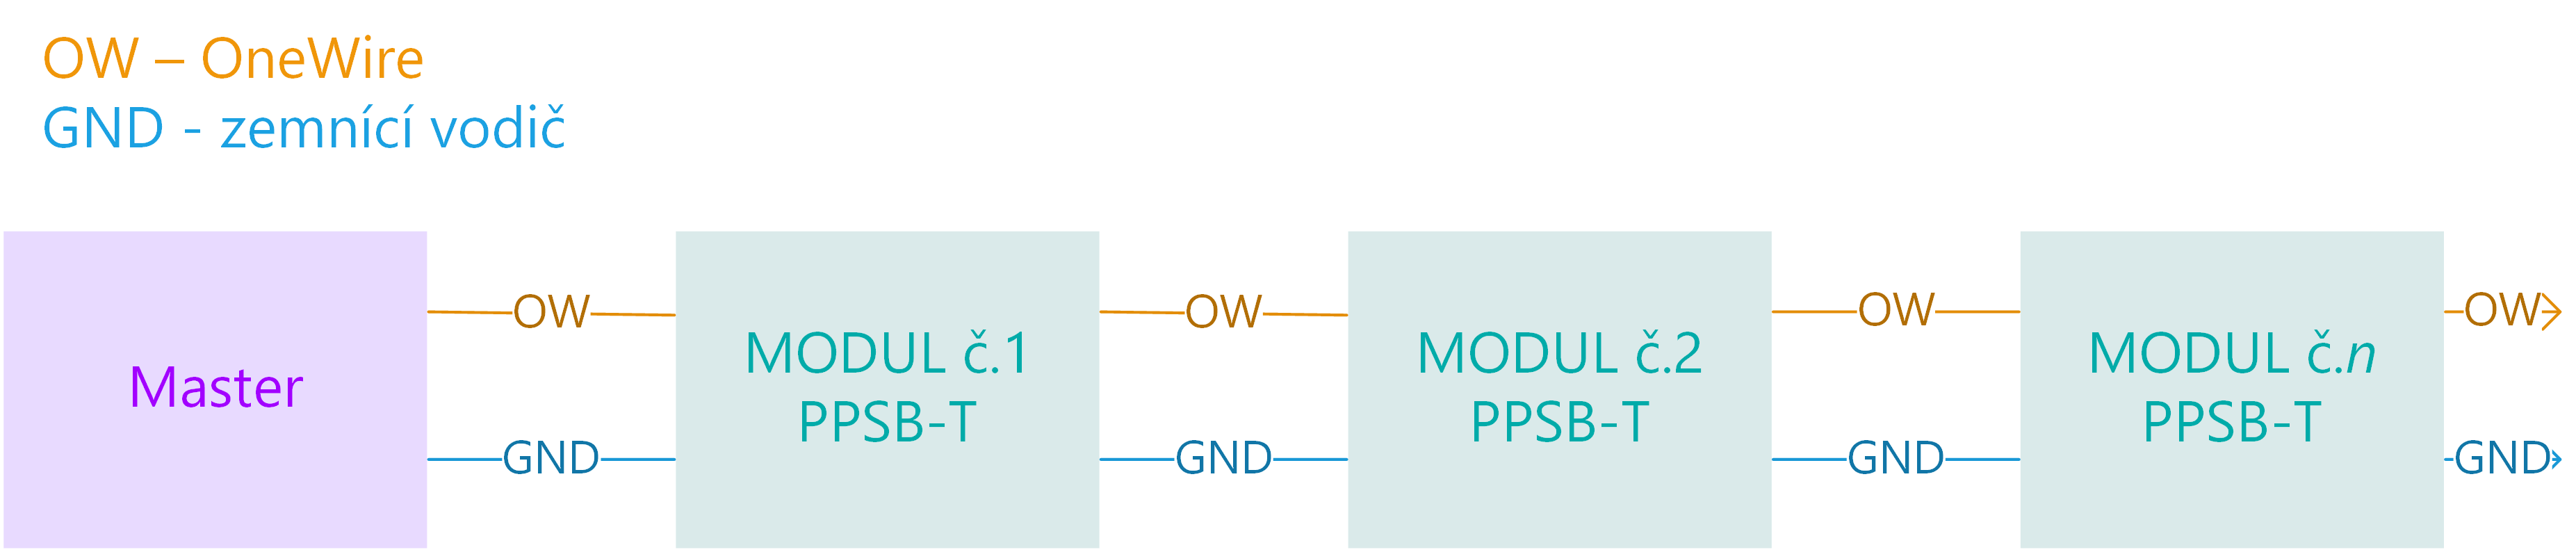
\includegraphics[width=\textwidth]{img/HARDWARE/PPSB-T_CHAIN.png}
   \caption{Řetězení desek PPSB-T.}
   \label{fig:PPSB-T_wiring}
\end{figure}

\noindent\B{PPSB-TH} osazena senzorem DHT22 \cite{DHT22} je schopna měřit vzdušnou vlhkost i teplotu.
Více o~tomto senzoru naleznete v~kapitole \ref{sec:DHT22}.
Narozdíl od PPSB-T tyto desky nelze řetězit.
Vizualizace naleznete na obrázku \ref{fig:PPSB-TH_VISUAL}.\newline

\section{Senzorika}
PROTOPlant primárně podporuje 3 typy senzorů. 
DS18B20 pro měření vzdušné teploty, DHT22 schopné měřit vlhkost i teplotu vzduchu a~senzory pro měření vlhkosti půdy.
DálePROTOPlant podporuje připojení senzorů vlhkosti půdy pracujících na bázi elektrické vodivosti.

\subsection{DS18B20}
\label{sec:DS18B20}
Senzory určené pro měření teploty. 
Komunikují po sběrnici OneWire (více v~\cite{DS18B20}, str. 4) vytvořené společností Maxim Integrated.
Jsou určeny pro teplotní rozsahy -55~\degree C až +125~\degree C.
V~měřícím rozsahu -10~\degree C až +85~\degree C jsou schopny měřit s~přesností na $\pm0,5$~\degree C.
K~PPCU je možno připojit až 30 těchto senzorů.

%\subsection{BME280}
%\label{sec:BME280}
%To be done.

\subsection{Senzory půdní vlhkosti}
\fxnote[author=PŠ]{Dopíšu během pondělka}

\subsection{DHT22}
\label{sec:DHT22}
Čidla, která měří vzdušnou vlhkost i teplotu.
Jejich přesnost je $\pm2\%$ relativní vlhkosti a~$\pm$0,5\degree C.
Opakovatelnost měření je poté $\pm$1\% relativní vlhkosti a~$\pm$0,2\degree C.
Tyto senzory komunikují jednosběrnicově, není tedy možno je řetězit.
K~PPCU je možno připojit těchto senzorů až 6.
Více viz \cite{DHT22}.

Do budoucna zvažuji přechod na senzory AM2321 \cite{AM2321} vzhledem k~tomu, že narozdíl od DHT22 dokáží komunikovat po sběrnici I\superscript{2}C (viz kapitola \ref{sec:I2C_comm}).

\newpage